\chapter{O Modelo de Objeto de Documentos (DOM)}

\begin{flushright}
  \textit{
    Todo mestre já foi aprendiz um dia. \\ Mas também engana-se quem pensa que a busca por \\  conhecimento tem um fim. 
  } \\
  
  \textbf{Autor desconhecido}
\end{flushright}

Você pode imaginar um documento HTML como um conjunto de caixas aninhadas. Tags como e encapsulam outras tags, as quais, por sua vez, contêm outras tags ou texto. Aqui está o documento de exemplo do último capítulo:

\begin{lstlisting}
	<html>
		<head>
			<title>Minha home page</title>
		</head>
		<body>
			<h1>Minha home page</h1>
			<p>Olá, eu sou Marijn e essa é minha home page.</p>
			<p>Eu também escrevi um livro! leia-o
			<a href="http://eloquentjavascript.net">aqui</a>.</p>
		</body>
	</html>
\end{lstlisting}

Essa página tem a seguinte estrutura:

\begin{figure}[H]
	\centering
	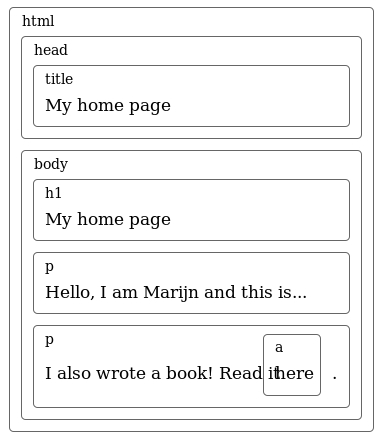
\includegraphics[scale=0.6]{imagens/html-boxes.jpg}
	\caption{Containers HTML}
	\legend{Fonte: \cite{haverbeke2014eloquent}}
\end{figure}

A estrutura de dados que o navegador usa para representar o documento segue este formato. Para cada caixa há um objeto, com o qual podemos interagir para descobrir coisas como: qual tag HTML ele representa e quais caixas e textos ele contém. Essa representação é chamada de Modelo de Objeto de Documentos, também apelidada de DOM (do inglês Document Object Model).

A variável global document nos dá acesso à esses objetos. Sua propriedade documentElement se refere ao objeto que representa a tag . Essa propriedade também nos fornece as propriedades head e body, alocando objetos para esses elementos.

Contudo, ao analisarmos a estrutura do HTML, podemos perceber que alguns elementos estão contidos dentro de outros, e assim, sucessivamente. Esse conjunto de elementos pode ser representado em formato de \textbf{árvore}, também conhecida como árvore DOM.

O DOM (Document Object Model), segundo \citeonline{Maldonado2018}  é uma interface que representa como os documentos HTML e XML são lidos pelo seu browser. Após o browser ler seu documento HTML, ele cria um objeto que faz uma representação estruturada do seu documento e define meios de como essa estrutura pode ser acessada. Nós podemos acessar e manipular o DOM com JavaScript, é a forma mais fácil e usada. 

\begin{figure}[H]
	\centering
	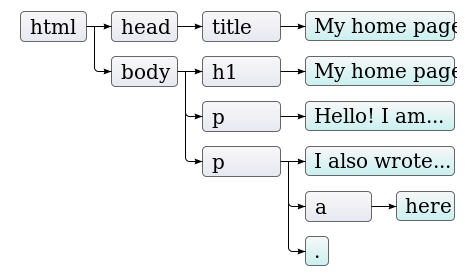
\includegraphics[scale=0.6]{imagens/html-tree.jpg}
	\caption{Árvore DOM}
	\legend{Fonte: \cite{haverbeke2014eloquent}}
\end{figure}

\section{Manipulando o DOM}

O DOM possui muitos métodos, são eles que fazem a ligação entre os nodes (elementos) e os eventos. O primeiro que veremos e o \textbf{write} e o \textbf{writeln}. 

Em nossas aulas, quando desejávamos mostrar um resultando, usávamos o console.log ou o alert. Contudo, por meio da manipulação do DOM, podemos printar esses dados diretamente na tela.

\begin{lstlisting}
	document.write("Hello World")
	document.writeln("Hello World")
\end{lstlisting}

Por meio dos comandos acima, todo o dom e limpo e apenas a palavra Hello World é printada na tela. 

\subsection{getElementById()}

Esse método retorna o elemento que estiver contendo o nome do ID passado. Como os IDs devem ser únicos, é um método muito útil para pegar apenas o elemento desejado.

\begin{lstlisting}
	 var idTag = document.getElementsById('idTag');
\end{lstlisting}

\textbf{Exemplo}

Neste exemplo veremos o evento OnClick. Não se preocupe, este será mais aprofundado nos próximos capítulos.

\begin{lstlisting}
	<html>
		<head>
			<title>getElementById example</title>
		</head>
		<body>
			<p id="para">Some text here</p>
			<button onclick="MudarCor('blue');">blue</button>
			<button onclick="MudarCor('red');">red</button>
		</body>
	</html>
\end{lstlisting}

\begin{lstlisting}
	function MudarCor(cor) {
		var elem = document.getElementById('para');
		elem.style.color = cor;
	}
\end{lstlisting}

\subsection{getElementsByClassName()}
	
Esse método retorna um \textbf{HTMLCollection} de todos elementos que estiverem contendo o nome da classe passada.

\begin{lstlisting}
	var x = document.getElementsByClassName("exemplo");
\end{lstlisting}

\begin{lstlisting}
	<!DOCTYPE html>
	<html>
		<body>
			<div class="exemplo">Primeiro nome</div>
			<div class="exemplo">Segundo nome</div>
			<button onclick="mudarTexto()">Try it</button>
			<script>
				function mudarTexto() {
					var x = document.getElementsByClassName("exemplo");
					x[0].innerHTML = "Novo texto";
				}
			</script>
		</body>
	</html>	
\end{lstlisting}